\documentclass[12pt,a4paper]{article}

\usepackage[a4paper, left=23mm, top=25mm]{geometry}
\usepackage{graphicx}
\usepackage[colorlinks=false]{hyperref}
\usepackage{url}
\usepackage{pdfpages}
\usepackage{pdflscape}


\title{CS351 Specification: Reliable Logic Using Unreliable Gates}
\author{Alia Meek, 2106850}
\date{}

\begin{document}
\maketitle


\section{Abstract}
An investigation into hardware solutions to tolerate faults, which can be based on particular architectures or error 
correcting codes (ECCs). Here, the project will investigate the options and build a simulation to demonstrate the 
operation of an established method.


\section{Problem}
As logic gates get smaller with increased transistor density, components are at the nanoscale where physical limits 
are approached with high levels of variability and manufacturing defects. At these limits, quantum mechanics comes 
into play: where electronic barriers were once thick enough to block current, they are now thin enough that electrons 
can simply ignore it -- a phenomenon known as \emph{quantum tunnelling}. It has been identified that by reducing the 
thickness of the \emph{gate oxide} -- a transistor component which electrically separates the gate (responsible for 
turning the transistor on and off) from the current-carrying channel -- to anything much less than a nanometre will 
result in too much current flowing across the channel when the transistor is “off”. This on its own, however, is 
only one of several leakage points, hence methods of fault tolerance are required.\cite{ref1}


\section{Objectives}
The objectives have been listed below, with a more detailed description of implementation given under 
\hyperref[sec:meth]{Methodology}.

\subsection{Essential}
These are the minimum requirements in order for the goals of the project to have been achieved.
\begin{itemize}
    \item Research the various proposed architectures and ECCs.
    \item Select a method of fault tolerance to simulate and fix a small error probability.
    \item Design an implementation of it in the chosen language.
    \item Perform benchmarking to analyse the trade off between accuracy and performance.
\end{itemize}

\subsection{Extension}
Given enough time left after completing the essential objectives, these features would enhance the quality of the 
project, but are not necessary for its successful completion.
\begin{itemize}
    \item Vary the error probability of the gates -- this will determine whether there are limits to the fault 
    tolerance of the chosen method and whether it is able to hold up to higher error probabilities
    \item Select another method to simulate and compare the relative effectiveness of each
\end{itemize}


\section{Methodology} \label{sec:meth}
In this project, we use the Von Neumann error model: a \emph{Von Neumann erroneous gate} is simply an ideal logic 
gate (one which never errors) cascaded with an error injecting XOR gate. The XOR gate takes a one as input with some 
probability $p$, called the \emph{gate error probability}, as well as the output from the ideal gate. \cite{ref2} 
This can be used to simulate the gate randomly inducing a bit flip. The chosen architecture or ECC will be 
implemented using these gates to determine how resilient it is to individual gate failures. \\

\noindent Since we are working with hardware, it makes sense to make use of a hardware description language (HDL) to 
simulate their behaviour. \texttt{SystemVerilog} is chosen here, over \texttt{Verilog}, owing to its ability to 
simulate electronic systems, as well as its support for datatypes such as enum, union, struct, string and class. It 
also allows for coverages design, which will ensure that test cases of interest (one gate errors, final gate errors, 
all gates error, etc.). Modules will be built to implement each of the gates, as well as the error probability. We 
can pass the error probability into the top-level module as a parameter, meaning it can be varied independent of the 
designed architecture. \\

\noindent A testbench will be designed to drive the module. Once this has been realised, simulation software will be 
used to gather data on the runtime of the simulated circuits. For control, we should run the module with no error 
correction, in order to get a baseline for runtime and error rate. To improve repeatability, simulations will be ran 
10 times, and the results averaged to get the mean runtime. These results can then be plotted. Simulation software 
does not typically have graphing capabilities; hence I now propose several alternative candidates for graphing.
\begin{itemize}
    \item \texttt{Python} has an extensive graphing library, \texttt{matplotlib}, which could be used to generate 
    the required graphs. \cite{ref3} Additionally, a further library, \texttt{openpyxl}, exists which can be used to 
    easily manipulate Excel spreadsheets. \cite{ref4}
    \item The code underpinning the \texttt{matplotlib} library is \texttt{MATLAB}, hence making it itself a strong 
    candidate for graph generation. Further, its import wizard would ease handling the spreadsheet as the data could 
    be simply imported into a \texttt{MATLAB} matrix, and the data plotted with minimal effort.
\end{itemize}

\noindent For each architecture and ECC simulated, I will look at two metrics: how high the gate error probability 
can be set before performance begins to fail, and the trade-off between any additional latency and the error 
correction performance. If time has allowed multiple methods to have been simulated, I will also compare their 
performances with each other.


\section{Resources \& Risks}
\subsection{Resources}
The project requires use of a computer and a simulation software capable of supporting \texttt{SystemVerilog}. At 
the time of writing, I have emailed the SCRTP facilities team to enquire if they have such software and whether I 
could be granted use, but they have not yet responded. In the event that either I am not given access, or they do 
not possess the software, I will look into acquiring a license myself.

\subsection{Risks}
The primary device that will be used during the project is my personal laptop, therefore, there is a risk of losing 
progress in the event of system failure. Using \texttt{git} and \texttt{GitHub} will not only allow the project to 
be downloaded onto another system, but it also provides version control in the event that work needs to be undone. 
To reduce the impact of data loss, the repository will be synced, at minimum, weekly with the local machine; though 
this may happen more frequently if waiting for a full week would increase the risk of significant loss (e.g., I was 
particularly productive on a day and complete a large portion of the code). Secondary machines capable of supporting 
the project are available in both the School of Engineering and Department of Computer Science Computer Labs.


\section{Legal, Social, Ethical and Professional Issues \& Considerations}
No such issues have been identified.


\begin{landscape}
    \section{Timetable}

    \noindent\centerline{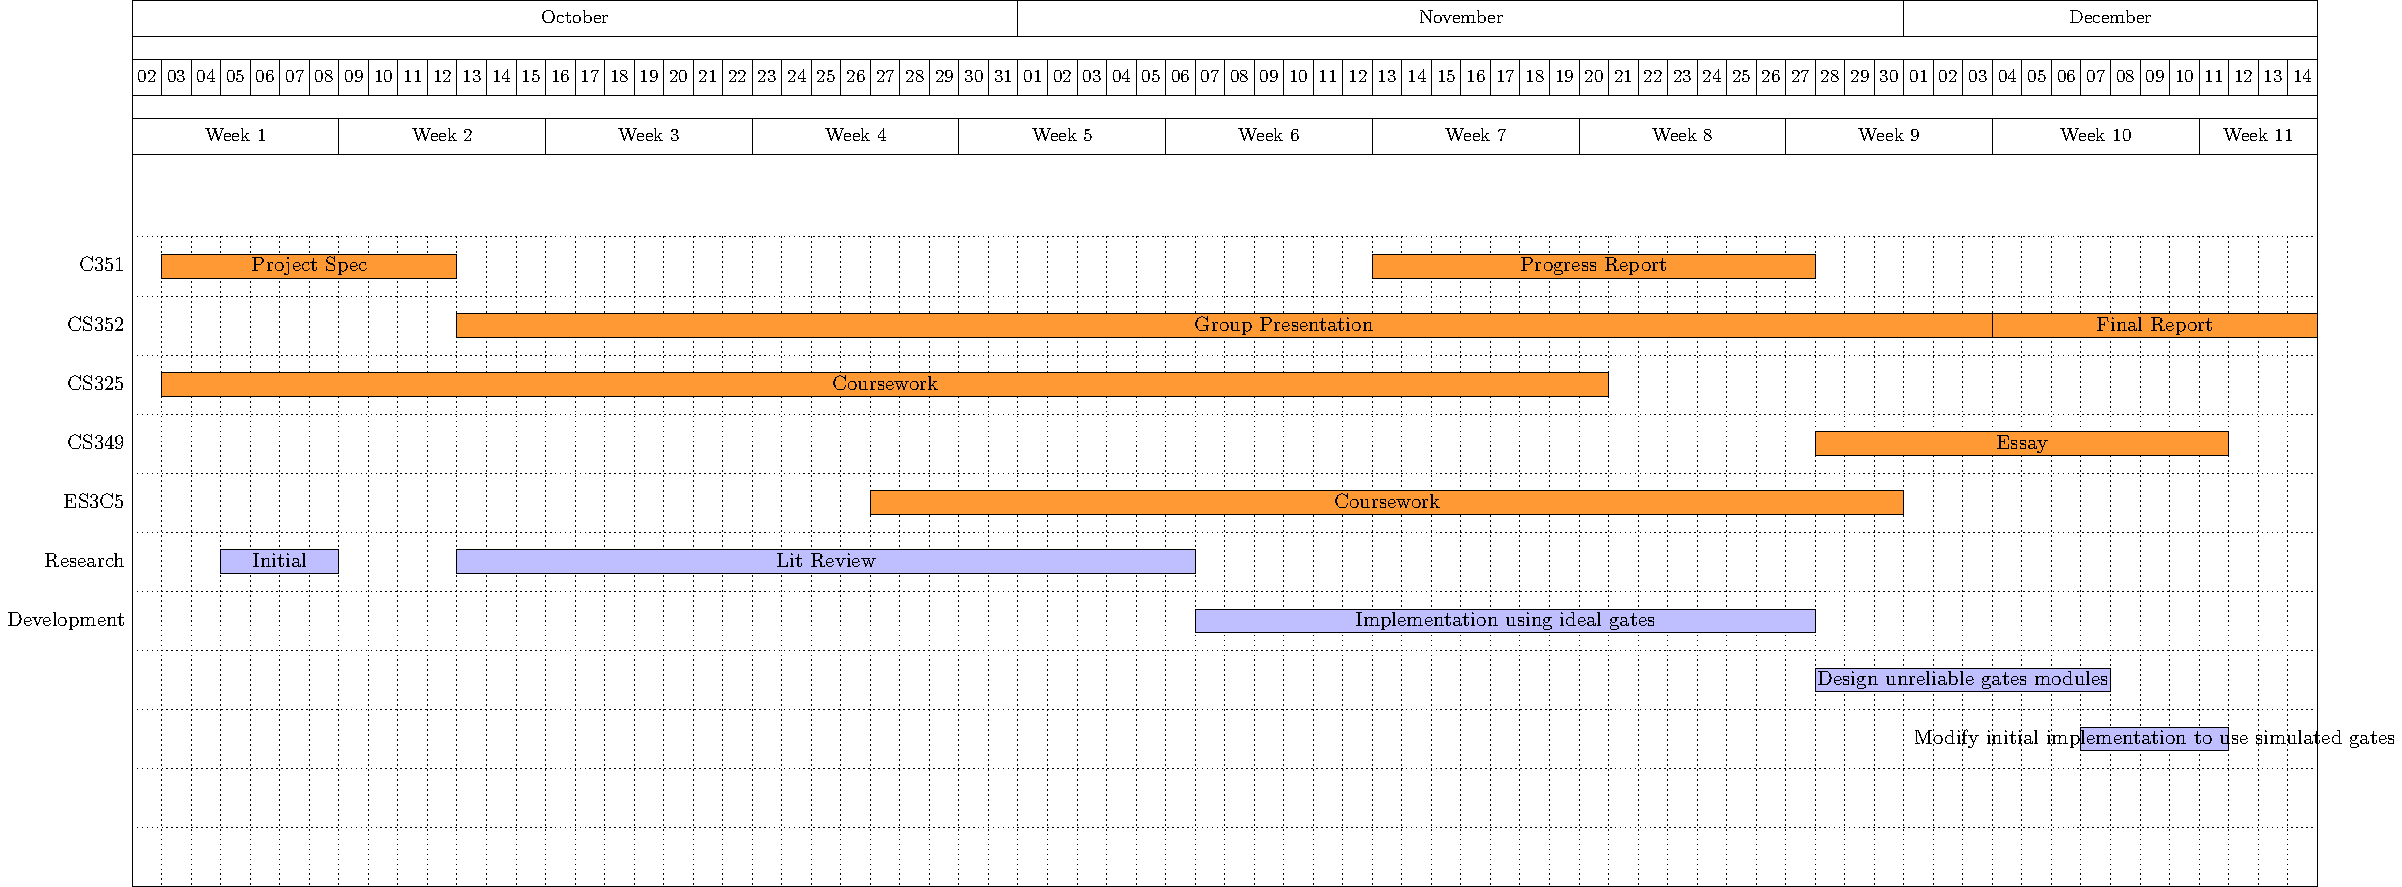
\includegraphics[scale=0.7]{chart.pdf}} \\

    \noindent The Christmas Holidays have been left for revision for an exam in week one of the second term. A 
    timetable for term two cannot be completely determined yet as not all deadlines have been set and delays in term 
    one may stall progress. The term will focus on continuing implementation of the model, as well as meeting any 
    extension objectives. In terms of deliverables, work on my presentation will begin in the first few weeks, 
    whereas I will begin my final report after the oral presentation has been given.
\end{landscape}


\bibliographystyle{ieeetr}
\bibliography{bibliography}

\end{document}